\documentclass[12pt,letterpaper,english,bibliography=totocnumbered,abstract=on]{scrartcl}

\usepackage{indentfirst}
\usepackage{appendix}
\usepackage{fullpage}
%\usepackage{subfiles}
\usepackage[T1]{fontenc}
\usepackage[latin9]{inputenc}
\usepackage{color}
\usepackage{babel}
\usepackage{verbatim}
\usepackage[unicode=true,pdfusetitle,
bookmarks=true,bookmarksnumbered=false,bookmarksopen=false,
breaklinks=true,pdfborder={0 0 0},pdfborderstyle={},backref=false,colorlinks=true]
{hyperref}
\hypersetup{linkcolor=blue,citecolor=blue,urlcolor=blue}

\usepackage{booktabs}
\usepackage{multirow}
\usepackage{adjustbox}
\usepackage{threeparttable}
\usepackage[table]{xcolor}
\usepackage{csquotes}
\usepackage{soul} % for hiliting text: \hl
% old style is authoryear
\usepackage[backend=biber, style=numeric, maxbibnames=99, sorting=none]{biblatex}
%\addbibresource{mylibrary.bib}
\addbibresource{CRB.bib}

% Use 'disable' as a parameter to hide todos
\usepackage[disable]{todonotes}
\usepackage{framed}

% Prevent page breaks within paragraphs
% https://tex.stackexchange.com/questions/21983/how-to-avoid-page-breaks-inside-paragraphs
%\widowpenalties 1 10000


\begin{document}
\titlehead{USDA-APHIS Progress Report}
\title{Coconut Rhinoceros Beetle Biological Control}
\author{Aubrey Moore, University of Guam}
\date{Submitted March 21, 2021}
\maketitle
\begin{description}	
	\item[Report ID:] AP19PPQS\&T00C168-PE-SA1-21 (RPT-51580)
	\item[Report Type:] Semiannual performance report
	\item[Performance Period:] August 8, 2019 - August 7, 2021
	\item[Federal Award Identification Number:] AP19PPQS\&T00C168
	\item[Agreement Title:] PPA7721 6R.0117.00 Guam CRB BC
\end{description}

\begin{footnotesize}
\url{https://github.com/aubreymoore/CRB-PPA19-Report3/raw/main/PPA19-report3.pdf}
\end{footnotesize}

\newpage{}
\tableofcontents{}

\todo[inline]{clean crap from source}
\listoftodos

\clearpage
\textbf{Notes for the Reader}
\begin{itemize}	
	\item This progress report covers August 2020 through March 2021.	
	\item Objectives and methods, as stated in the approved work plan \cite{mooreWorkPlanAPHISPPA2020} are presented in a frame at the start of each section. 	
	\item The University of Guam CRB biological control project is a long-term effort supported by multiple short-term grants. Some of the activities reported here have been partially funded by sources external to the FY19 APHIS-PPA CRB Biocontrol grant.  	
\end{itemize}


\newpage

\begin{framed}
\section{Objective 1: CRB Control}

The primary objective is to find an \textit{Oryctes rhinoceros} nudivirus (OrNV) isolate which can be used as a highly effective biological control agent for long-term suppression of CRB-G populations. As soon as laboratory studies indicate discovery of an OrNV isolate which is a potential biological control agent for CRB, we will multiply the virus \textit{in vivo} and initiate field releases under the conditions of an existing USDA-APHIS permit.
\end{framed}

We have attained little progress towards completing our primary objective, which is to find an isolate of OrNV which is a promising candidate for biocontrol of CRB-G, because of COVID-19 travel restrictions and technical problems with our bioassays. Impediments towards progress are discussed in detail in Section \ref{impediments}.

\newpage
\begin{framed}
\subsection{Regional Collaboration}

Work will continue with colleagues at AgResearch New Zealand, the Secretariat of the Pacific Community (SPC), Tokyo University, the University of Hawaii and others to put together a regional collaboration with the objective of finding an effective biocontrol agent for CRB-G.

\subsubsection{Methods}

\begin{itemize}
    \item Moore and Grasela will participate in the CRB-G biocontrol meeting at the IAPPS meeting in Hyderabad, India, November 2019.
    \item Moore will continue to maintain a web site to facilitate exchange of information on CRB-G biocontrol.
\end{itemize}
\end{framed}

\subsubsection{Progress}

Project staff promoted Pacific-wide collaboration among people trying to find solutions to the CRB problem by helping to organize professional meetings and by providing online tools to facilitate sharing of scientific and technical information.

\paragraph{CRB Action Group Meeting; December 9, 2020}
This meeting was run as a Zoom webinar hosted by the University of Guam. A recording is available online.\cite{mooreVideoRecordingCRBG2021}

\subparagraph{Agenda and Presentations:}

\begin{itemize}
	\item Regional Reports
	\item \textbf{Aubrey Moore}: Automated roadside video surveys for detecting and monitoring CRB damage to coconut palms. \cite{mooreAutomatedRoadsideVideo2020}
	\item \textbf{Sarah Mansfield}: Bioassays with OrNV: Progress and pitfalls.
	\item \textbf{Madoka Nakai and Shunsuke Tanaka}: Characterization of a Palauan isolate of \textit{Oryctes rhinoceros} nudivirus (OrNV).
	\item \textbf{Kayvan Etebari}: Transcriptomic responses of different geographical populations of coconut rhinoceros beetles to \textit{Oryctes rhinoceros} nudivirus (OrNV) infection.
	\item Open Discussion	
\end{itemize}


\paragraph{CRB Action Group Meeting; March 17, 2021}
This meeting was run as a Zoom webinar hosted by the University of Guam. A recording is available online \cite{mooreVideoRecordingCRBG2020}.

\subparagraph{Agenda and Presentations:}
\begin{itemize}
	\item Regional Reports
	\item \textbf{Sulav Paudel}: Review paper on biological control of CRB
	\item \textbf{Mark Ero}: Evaluation of CRB-G pheromone from the Solomon Islands
	\item \textbf{Lastus Kuniata}: Insecticide work in young oil palm in Solomon Islands
	\item \textbf{Katayo Sagata}: Evaluation of integrated management options in an oil palm cropping system in PNG
	\item Open Discussion	
\end{itemize}


\paragraph{Rota CRB Eradication Program}
The PI made a presentation in a webinar organized by Department of the Interior - Office of Insular Affairs (DOI-OIA) entitled \textit{CRB Biology: Know Your Enemy} \cite{mooreCRBBiologyKnow2021}. This webinar will be converted into a podcast and published online by DOI-OIA which is supporting the Rota CRB Eradication Project with a \$250,000 grant.

\paragraph{LISTSERV}
The PI established a LISTSERV to facilitate email discussions among members of the CRB Action Group.\cite{mooreOnlineEmailDiscussion2021}

\paragraph{Online CRB Reference Library}
Project staff maintain an online reference library of technical and scientific information about coconut rhinoceros beetle.\cite{mooreOnlineReferenceLibrary2021}


\newpage
\begin{framed}
\subsection{Foreign Exploration for an Effective Biocontrol Agent for CRB-G}

Foreign exploration in search of a microbial biocontrol agent for CRB-G is already underway. During January, 2017, Moore, Iriarte and Marshall collected an isolate if OrNV from a CRB-G population in Negros Island, Philippines. Laboratory bioassays indicate that this isolate is not a good candidate for biocontrol.

We are currently performing laboratory bioassays to evaluate two novel isolates obtained from AgResearch New Zealand. In addition we are attempting to isolate OrNV from CRB adults collected in Taiwan. This population was targeted because Dr. Shizu Watanabe, University of Hawaii, reported an 82\% OrNV infection rate in CRB-G collected from this island.

Our next target population is CRB-G found on the southern islands of Japan. We plan to collaborate with Dr. Madoka Nakai, Tokyo University of Agriculture and Technology, to obtain CRB-G/OrNV specimens from these islands.

\subsubsection{Methods}

\begin{itemize}
	\item Subsamples of CRB collected during foreign exploration will be shipped to AgResearch New Zealand to determine CRB biotype and to isolate OrNV
	\item OrNV isolates collected during foreign exploration will be tested in the insect pathology lab at UOG using standard bioassay protocols.
	\item The PI and insect pathology post-doc will travel to Japan to collect CRB-G and OrNV. 
\end{itemize}
\end{framed}

\subsubsection{Progress}

The project applied for and was granted USDA-APHIS permits to import \textit{Oryctes rhinoceros} \cite{usda-aphis_crb_2019} and \textit{Oryctes rhinoceros} nudivirus (OrNV) \cite{usda-aphisImportPermitOrNV2020}.

No progress was made on foreign exploration for OrNV isolates as potential biocontrol agents for CRB during the period covered by this report because of COVID-19 travel restrictions. See section \ref{covid} for details.

\newpage
\begin{framed}
\subsection{Establish Lab Colonies of CRB-G and CRB-S}

We will establish sustainable laboratory colonies of CRB-G and virus susceptible beetles (CRB-S) as a source of healthy beetles for bioassays.

Note: Establishment of a CRB-S colony is contingent on receiving a USDA-APHIS import permit to import live coconut rhinoceros beetles. I requested a permit on March 19, 2019 (Application number P526-190319-001) to replace a previous permit, P526P-11-01844, which I accidentally allowed to lapse into oblivion after only one shipment.

If we are allowed to import CRB-S, this will allow us to do comparative studies to:

\begin{itemize}
\item Measure difference in susceptibility to OrNV isolates. (Resistance of CRB-G to OrNV has not yet actually been proven by comparative bioassays.)
\item Test for behavioral differences. (It has been hypothesized that the aggregation pheromone, oryctalure, is less attractive to CRB-G than CRB-S.)
\end{itemize}

\subsubsection{Methods}

\begin{itemize}
	\item Larvae and adults will be reared individually in Mason jars enclosed by metal caps. Larvae will be fed a store-bought steer manure/soil blend on which we have reared CRB larvae for many years. Adults will be bedded in peat moss and fed banana slices weekly.
	\item Mason jars will be placed in environmental cabinets set at 30 deg. C, 80\% RH and 12 h photoperiod.
	\item Detailed records for each individual beetle will be stored in an existing online laboratory information management system (LIMS). These data will be made available to USDA-APHIS.
\end{itemize}
\end{framed}

\subsubsection{Progress}



The project applied for and was granted a USDA-APHIS permit to import \textit{Oryctes rhinoceros},Biotype CRB-S \cite{usda-aphis_crb_2019}, \cite{moore_additional_2019}.

No progress was made on establishing laboratory colonies for CRB-G and CRB-S biotypes during the period covered by this report because of COVID-19 travel restrictions and University of Guam closures. See section \ref{covid} and section \ref{stayathome} for details.


\newpage\begin{framed}
\section{Objective 2: Establish a Sustainable Coconut Palm Health Monitoring System}

The CRB-G outbreak on Guam is currently unmonitored on an island-wide basis. An island-wide pheromone trapping system, using about 1500 traps, was operated by the University of Guam from 2008 to 2014. This monitoring system was transferred to the Guam Department of Agriculture which abandoned the effort at the end of February, 2016.

Currently, many coconut palms are being killed by CRB-G. But, in the absence of a monitoring system, we do not have an estimate of tree mortality or whether or not the damage is increasing or decreasing. Clearly, establishment of a monitoring system is necessary if we want to evaluate success of the proposed biocontrol project, or any other mitigation efforts.

Rather than re-establish a trapping survey, we intend to establish a monitoring system to track temporal and spatial changes in the extent of CRB damage to Guam's coconut palms. Damage symptoms such as v-shaped cuts to fronds, bore holes, and dead standing coconut palm stems are readily observed during roadside surveys. Survey data will be collected using a digital video camera mounted on a truck. Initially, video images of coconut palm damage by CRB-G will be detected, classified and tagged by a technician. When a large number of images have been tagged, these will be used to train a fully automated CRB damage detection and monitoring system. This automated system may be useful as an early detection device for CRB. Roadside surveys on Guam will be performed bimonthly.

\subsubsection{Methods}

\begin{itemize}
	\item A protocol will be developed to perform roadside surveys of CRB damage. Damage will be recorded using videos recorded by a vehicle-mounted Olympus TG-5 camera. This camera records GPS coordinates.
	\item Videos will be tagged using the open source Computer Vision Annotation Tool (CVAT).
	\item An object detector which locates and classifies CRB damage in video recordings will be trained using annotated videos from the previous step. We intend to use the TensorFlow implementation of the Faster R-CNN Deep Learning model. Training a CRB damage detector using deep learning requires use of a computer with specialized software (TensorFlow) and specialized hardware (a graphics processing unit (GPU)). Instead of purchasing a physical machine we will rent a virtual machine designed specifically for this application from Amazon Web Services.
	\item Results from the trained object detector will be evaluated using the human annotated videos.
	\item We will develop an automated processing system which takes roadside videos as input and generates CRB damage maps as output.
\end{itemize}
\end{framed}

\subsubsection{Progress}

Bimonthly automated roadside video surveys for CRB damage are now operational on Guam and the system has been tested on Rota. Videos recorded with a smart phone attached to a vehicle are analyzed using custom-designed artificial intelligence software which recognizes coconut palms and measures CRB damage. A nontechnical description of the survey method is given in the next section.

A presentation on this new CRB survey methodology was made at the December 9 2020 meeting of the CRB-G Action Group conducted as a Zoom webinar \cite{mooreVideoRecordingCRBG2020}, \cite{mooreAutomatedRoadsideVideo2020}.

\paragraph{Guam Roadside Video Survey 1}

The following four images were extracted from a draft of the University of Guam's Western Pacific Tropical Research Center impact report for 2020. They provide a nontechnical overview of the new automated roadside video survey for CRB damage and results from the first Guam survey in October, 2020.

\begin{figure}[h]
	\centering
	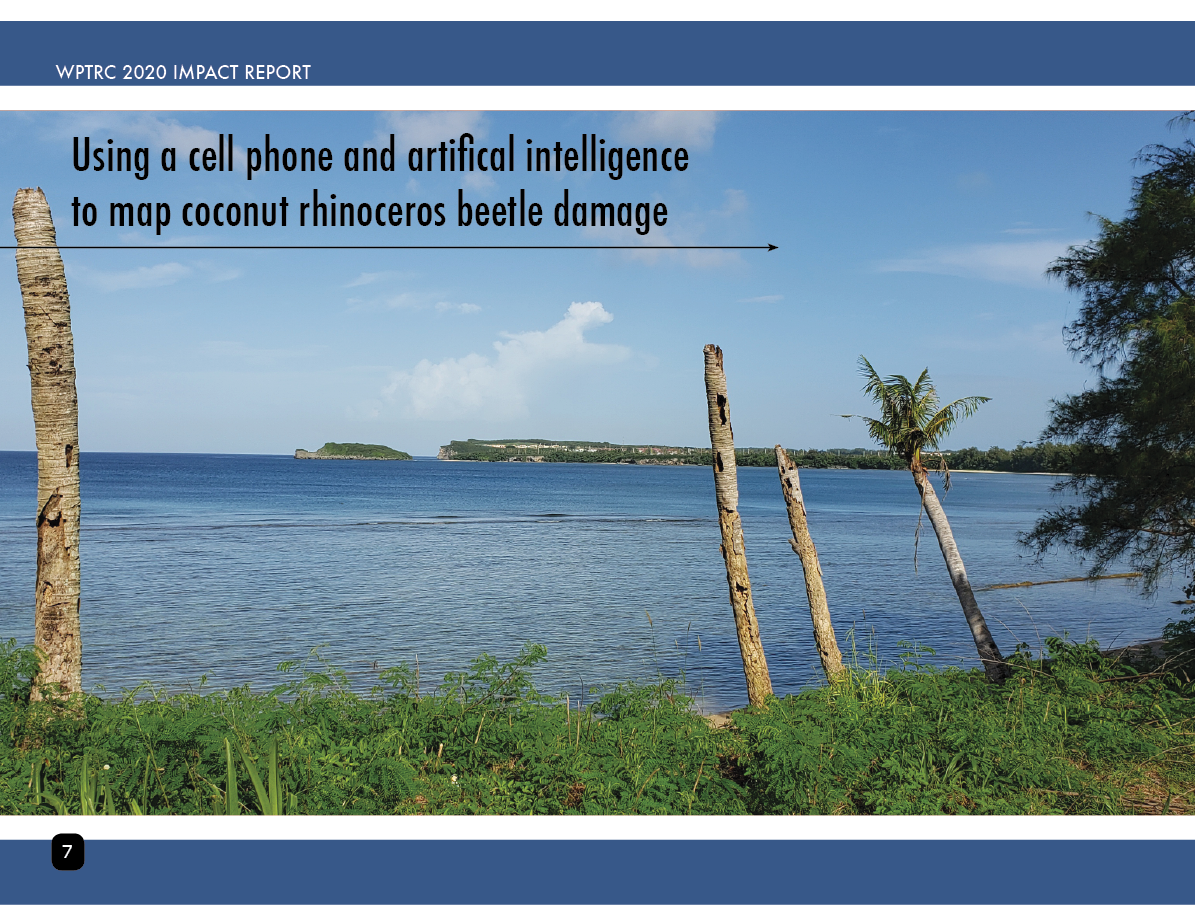
\includegraphics[width=1\linewidth]{images/impact-report07.png}
	\caption{Feature article in the University of Guam's Western Pacific Tropical Research Center impact report for 2020.}
	\label{fig:roadside1-1}
\end{figure}

\begin{figure}[h]
	\centering
	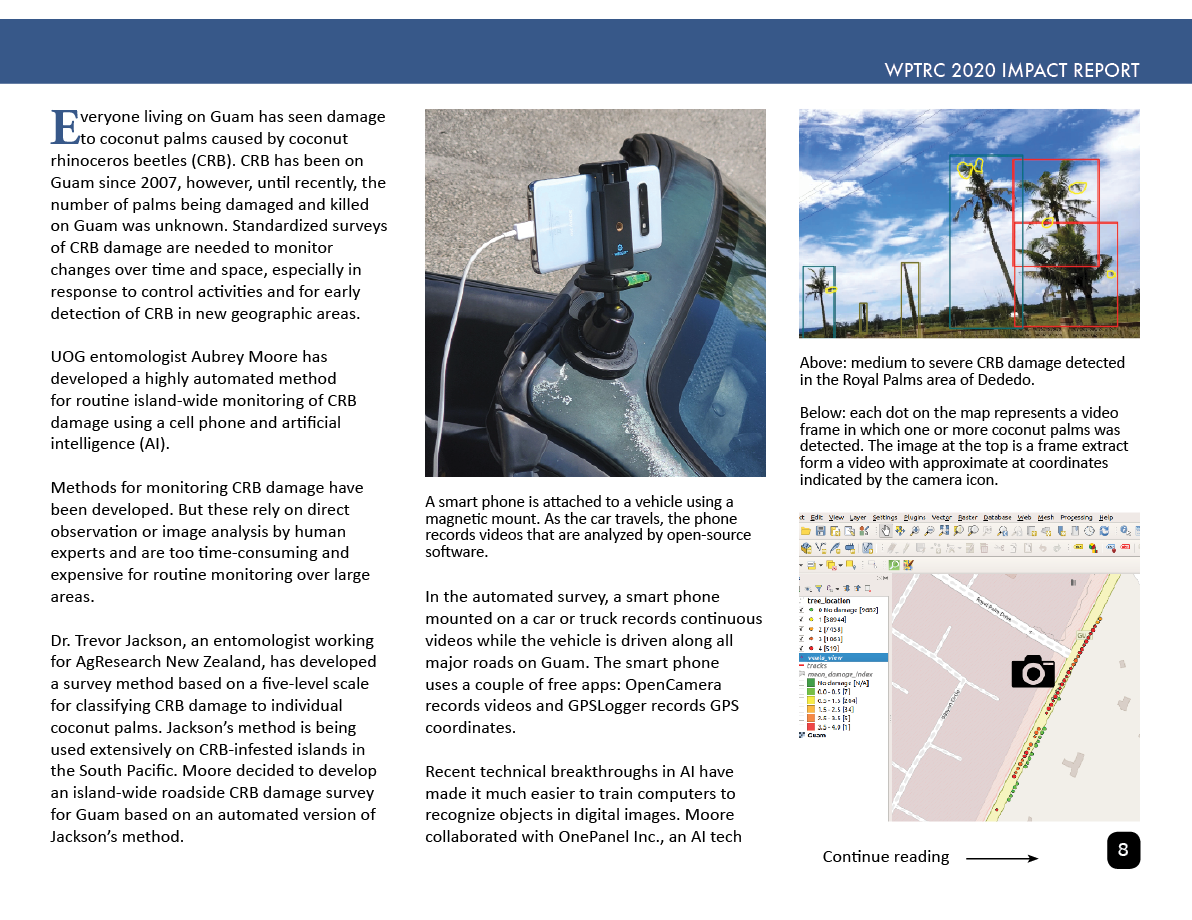
\includegraphics[width=1\linewidth]{images/impact-report08.png}
	\caption{[Continued] Feature article in the University of Guam's Western Pacific Tropical Research Center impact report for 2020.}
	\label{fig:roadside1-2}
\end{figure}

\begin{figure}[h]
	\centering
	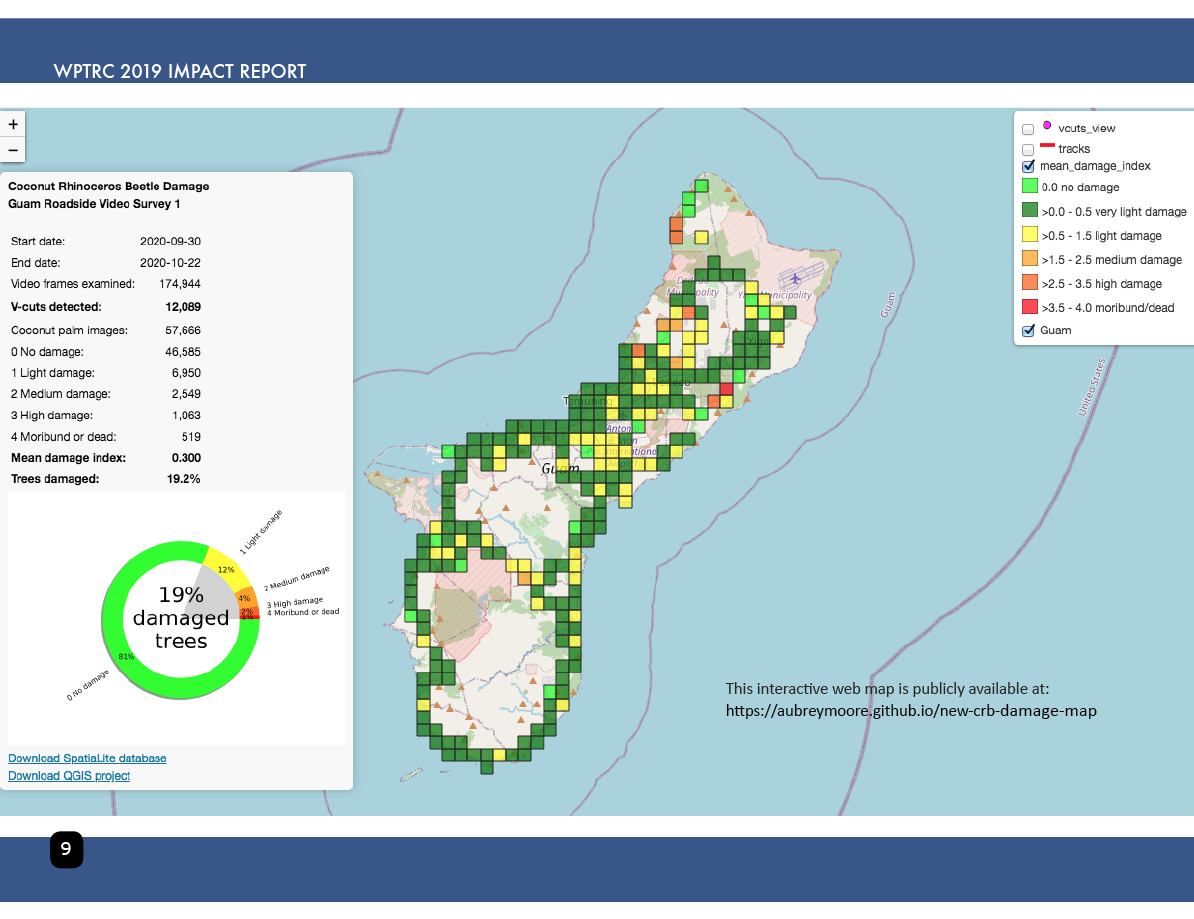
\includegraphics[width=1\linewidth]{images/impact-report09.png}
	\caption{[Continued] Feature article in the University of Guam's Western Pacific Tropical Research Center impact report for 2020. This interactive web map is publicly available at: \url{https://aubreymoore.github.io/new-crb-damage-map}}
	\label{fig:roadside1-3}
\end{figure}

\begin{figure}[h]
	\centering
	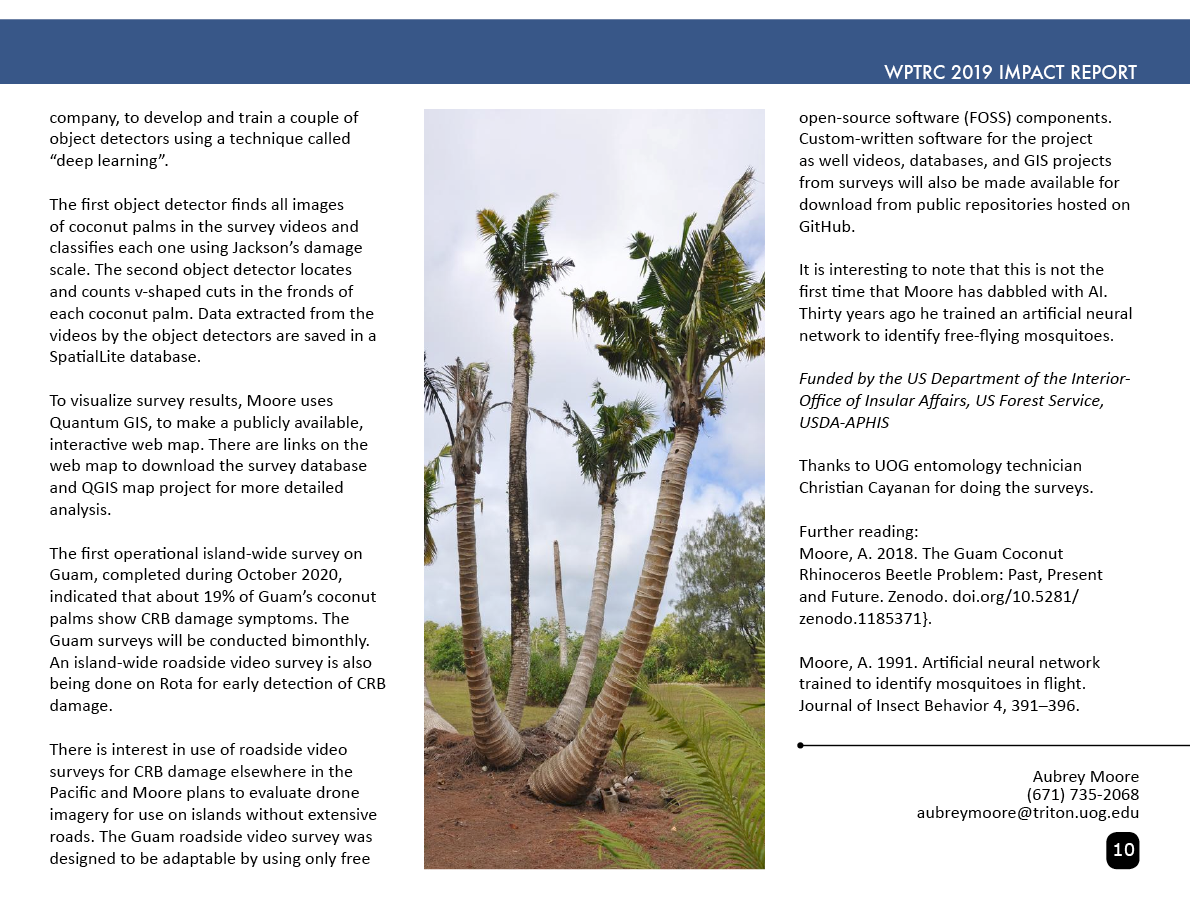
\includegraphics[width=1\linewidth]{images/impact-report10.png}
	\caption{[Continued] Feature article in the University of Guam's Western Pacific Tropical Research Center impact report for 2020.}
	\label{fig:roadside1-4}
\end{figure}

\clearpage
\paragraph{Guam Roadside Video Survey 2}

The proportion of coconut palms damaged by CRB increased significantly from 19.2\% in
October 2020 to 21.5\% in December 2020 (p < 0.001; Fisher's exact test).

\begin{figure}[h]
	\centering
	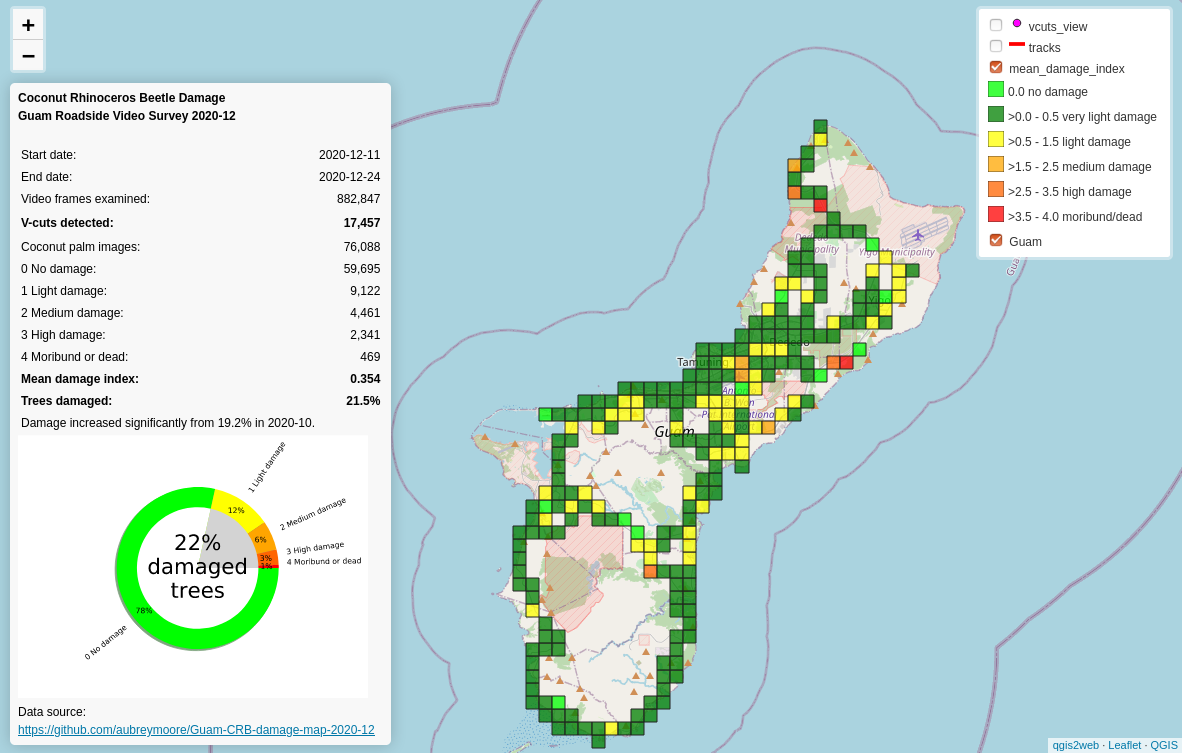
\includegraphics[width=1\linewidth]{images/crb-webmap-2020-12.png}
	\caption{Screenshot of an interactive web map of results from a roadside video survey of
		CRB damage on Guam in December 2020 \url{https://aubreymoore.github.io/Guam-CRB-damage-map-2020-12/webmap/v1/}.}
	\label{fig:guam02}
\end{figure}


\clearpage
\paragraph{Rota Roadside Video Survey 1}

Rota was invaded by CRB in 2017 and eradication efforts by Rota Department of Land and Natural Resources have successfully kept the population at a very low level, although the population has begun to spread to new areas of the island. In October 2020, a smart phone and associated equipment was sent to Rota-DLNR so that they could do an initial roadside video survey in support of their CRB control efforts. In addition to the equipment, a survey setup guide and  \cite{aubreymooreSetAutomatedRoadside2020} and a setup video \cite{mooreYouTubeVideoMounting2020} were prepared and sent.

The survey was performed by Mark Manglona, Rota-DLNR and the phone containing videos from the survey was returned to the University of Guam.  Videos were analyzed using the workflow developed for the Guam surveys. The resulting web map contained many false positives for CRB damage, but there is one hit which shows a classic v-shaped cut probably caused by CRB. For convenience, data for this hit (images, date, location) were documented as an iNaturalist observation (Figure \ref{fig:rota-inat-obs}). If this v-shaped cut was caused by CRB, there will be a bore hole. Rota-DLNR located the damaged palm but did not find a bore hole.  Therefor the damage was not caused by CRB.


\begin{figure}[h]
	\centering
	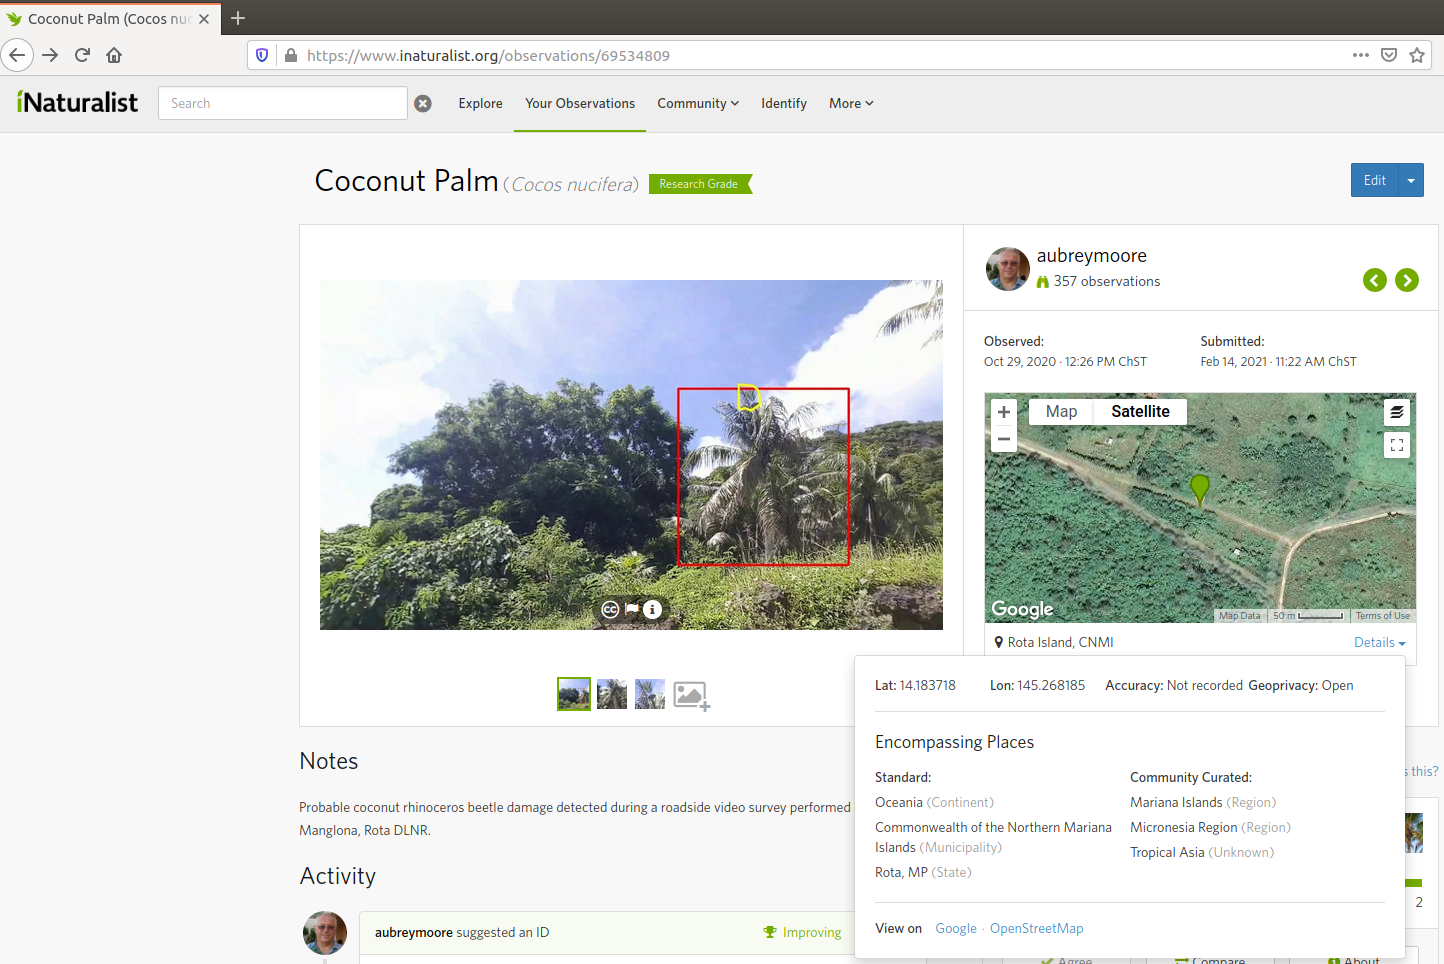
\includegraphics[width=1\linewidth]{images/Rota-iNat-obs}
	\caption{Screenshot of an iNaturalist observation documenting possible coconut rhinoceros beetle damage detected during a roadside video survey performed by Rota DLNR. \url{https://www.inaturalist.org/observations/69534809}.}
	\label{fig:rota-inat-obs}
\end{figure}

\newpage




\section{Impediments to Progress in the Guam CRB Biocontrol Program}
\label{impediments}
Significant progress was made on the Damage Survey and Regional Collaboration
components of this grant. However, progress on the Biological Control component is
lagging because of travel restrictions, stay at home orders, and a major technical problem.

\subsection{Delays Caused by Travel Restrictions}
\label{covid}

The original work plan included foreign travel to collect novel OrNV isolates for evaluation
as biocontrol agents and to collect virus susceptible CRB biotypes for comparative bioassays.
Our first planned collecting trip was to visit American Samoa in December 2019. This trip
was canceled at the last minute because of a measles outbreak. Our second attempt, in
March 2020 was also canceled at the last minute, because of COVID-19 travel restrictions.

\subsection{Delays Caused by COVID-19 Stay-at-Home Orders and University Closures}
\label{stayathome}
Progress was further delayed by Government of Guam stay at home orders. The University
of Guam was officially closed from March 20 to May 10 2020 and again from August 16 2020
to January 15 2021.

\subsection{Delays Caused by Detection of OrNV in CRB Collected on Guam}

Our lab currently uses CRB-G adults collected from pheromone traps as test animals
in bioassays evaluating OrNV isolates as biocontrol agents under the assumption that the
Guam beetle population contains only the CRB-G biotype and is free from OrNV infection.
In 2019 we gained the capacity to perform PCR in our lab began testing these assumptions.
PCR results indicated that field-collected beetles were all CRB-G, but 18\% of these tested
positive for OrNV.

Based on these results, the PI decided to suspend bioassays until we had conclusive evidence of OrNV infection in the Guam CRB-G population. An experimental plan \cite{mooreExperimentalPlanDetermining2020} was
developed and executed. One hundred beetles were collected from each of two trapping sites
(Leo Palace Resort in Southern Guam and the UOG Ag. Expt. Stn. in northern Guam).
Gut samples were obtained from these beetles and tested using PCR in our lab and also in
Sean Marshall's lab at AgResearch New Zealand. In PCR results from both labs all beetles tested positive for CRB-G biotype and negative for OrNV infection \cite{graselaInvestigationDeterminePresence2020}. We suspect that
previous OrNV positive tests were the result of lab contamination (not false positives).
During the hiatus in OrNV bioassays, we re-examined our bioassay methodology and have
decided to make major changes before moving forward:

\paragraph{Re-establishment of a CRB rearing program.} High variance among results from bioassay
replicates and high mortality rates are a serious impediment to progress in finding an
OrNV isolate which can be used as an effective biocontrol agent for CRB-G. Beetles
collected from pheromone traps are not ideal test insects because they vary in age and
many are infected with \textit{Metarhizium majus}.
We intend to re-establish the Guam CRB rearing program to supply healthy, standardized test insects. Insects will be reared individually in Mason jars and a detailed record
will be maintained for each individual. Larvae will be fed a diet of heat-sterilized CRB
breeding site material from dead standing coconut trunks. The CRB-G lab colony will
be initiated with surface-sterilized eggs and isofemale lineages will be maintained.
Because the life cycle of the coconut rhinoceros beetle is about 9 months, there will
be a lag time of about one year before the rearing program is fully operational and bioassays can resume.

\paragraph{Measurement of sublethal impacts of OrNV infection.} The literature indicates
that reduction in damage to coconut palms after release of OrNV may be the result of
sublethal impacts on the population rather than mortality. These impacts may include
reduction in fecundity, feeding, and flight. Bioassays which measure only mortality may
reject promising biocontrol candidates.
We already indirectly track feeding by weighing beetles during bioassays but will also
include egg counts in future observations so that we can measure changes in fecundity. We are also considering using flight mills to measure flight capability.

\paragraph{Acquisition of virus susceptible biotypes.} One or more lab colonies of virus-susceptible biotypes are required for comparative bioassays. We
originally planned to source non-CRB-G beetles during foreign exploration for OrNV
isolates, but this has not happened because of COVID-19 travel restrictions.
Our new plan is to import gravid females from places such as Palau, where one or more
virus-susceptible biotypes are known to exist, in addition to CRB-G. Eggs from these
females will be used to establish isofemale lineages and these lines will be genotyped
using DNA extracted from the imported females.

\clearpage
\printbibliography[heading=bibintoc]

\end{document}
